V tejto kapitole sa oboznámime so základnými pojmami z bioinformatiky a
niektorými dátovými štruktúrami a algoritmami, ktoré budú neskôr použité pri
implementácii.

\section{Formálne definície a označenia}
\label{sec:formalne_definicie}

\begin{defn}
Abeceda je konečná neprázdna množina symbolov (písmen). Označujeme ju $\Sigma$.
\end{defn}

\begin{pozn}
V našom kontexte bude pracovať s abecedou $\Sigma=\{A, C, T, G\}$.
\end{pozn}

\begin{defn}
Reťazec nad abecedou $\Sigma$ je konečná postupnosť symbolov z $\Sigma$.
\end{defn}

\begin{defn}
Dĺžka reťazca je dĺžka postupnosti, ktorá ho vytvára. Dĺžku reťazca $s$ označujeme $|s|$.
\end{defn}

\begin{defn}
Podreťazcom reťazca $s=a_0 a_1 \ldots a_n$ je súvislá podpostupnosť $t=a_i a_{i+1} \ldots a_j$, pričom platí $0 \leq i \leq j \leq n$. Takýto podreťazec označujeme $t=s[i,j]$. Špeciálne, ak $i=0$, tak takýto podreťazec nazývame prefix a ak $j=n$, tak sufix reťazca $s$.
\end{defn}

\begin{ozn}
I-ty symbol postupnosti tvoriacej reťazec $s$ budeme označovať $s[i]$.
\end{ozn}

\begin{defn}
K-merom nazývame ľubovoľný podreťazec dĺžky $k$ ľubovoľného reťazca $s$ z množiny reťazcov $S$.
\end{defn}

\todo{mozno zmazat definiciu zarovnania, lebo je to tu kus odveci}

\begin{defn}
    Zarovnanie sekvencií $S_0=a_1 a_2 \ldots a_n$ a $S_1 = b_1 b_2 \ldots b_m$ je funkcia $f : \mathbb{Z}_n \to \mathbb{Z}_m \cup \{ \bot \} $ spĺňajúca nasledovnú podmienku:
        
    $ (\forall i, j \in \mathbb{Z}_n) (f(i) \neq \bot \wedge f(j) \neq \bot \wedge i < j) \implies (f(i) < f(j)) $
\end{defn}
    
\bigskip
    
\begin{example}
    Dve možné zarovnania sekvencií $S_0$ = \texttt{AGGTA} a $S_1$ = \texttt{GCTA}:
    
    \bigskip
    
    \begin{minipage}{2.5in}
        \begin{tabular}{ c c c c c c c }
            0 & 1 & 2 &   & 3 & 4 \\ \hline     
            A & G & G & - & T & A \\
            - & G & - & C & T & A \\ \hline
              & 0 &   & 1 & 2 & 3 \\   
        \end{tabular}
    \end{minipage}
    \begin{minipage}{2.5in}
        \begin{tabular}{ | c | c | }
            \hline            
            $i$ & $f(i)$ \\ \hline             
            0   & $\bot$ \\ \hline 
            1   & 0      \\ \hline
            2   & $\bot$ \\ \hline
            3   & 2      \\ \hline
            4   & 3      \\ \hline
        \end{tabular}
    \end{minipage}
        
    \bigskip
        
    \begin{minipage}{2.5in}
        \begin{tabular}{ c c c c c c c c c }
            0 & 1 & 2 & 3 & 4 &           \\ \hline     
            A & G & G & T & A & - & - & - \\
            - & - & G & - & - & C & T & A \\ \hline
            &   & 0 &   &   & 1 & 2 & 3 \\   
        \end{tabular}
    \end{minipage}
    \begin{minipage}{2.5in}
        \begin{tabular}{ | c | c | }
            \hline            
            $i$ & $f(i)$ \\ \hline             
            0   & $\bot$ \\ \hline 
            1   & $\bot$ \\ \hline
            2   & 0      \\ \hline
            3   & $\bot$ \\ \hline
            4   & $\bot$ \\ \hline
        \end{tabular}
    \end{minipage}        
\end{example}
    
\bigskip

\begin{defn}
    \label{def:reverzny_komplement}
    Reverzným komplementom reťazca $S=a_0a_1 \ldots a_{n-1}$, kde \\
    $\forall i \in \mathbb{N} : 0 \leq i < n : a_i \in \{A, C, T, G\}$ je reťazec $S_{rc}=b_0b_1 \ldots b_{n-1}$, pre ktorý platí:
    $$
    \forall i \in \mathbb{N} : 0 \leq i < n : b_i = \begin{cases}
                                                        A : a_{n-i-1} = T \\
                                                        T : a_{n-i-1} = A \\
                                                        C : a_{n-i-1} = G \\
                                                        G : a_{n-i-1} = C  
                                                    \end{cases}
    $$
\end{defn}

\begin{example}
    Pre reťazec $S=ACTTTGCCCT$ je reverzným komplementom reťazec $S_{rc}=AGGGCAAAGT$.
\end{example}

\section{Sekvenovanie}
\label{sec:sekvenovanie}
Sekvenovanie DNA je súhrnný termín pre biochemické metódy, pomocou ktorých sa zisťuje poradie nukleotidov (A, C, T, G) v sekvenciách DNA. Tieto metódy nedokážu prečítať celý genóm naraz, ale len po malých častiach. 

Z informatického pohľadu je výsledkom sekvenovania DNA sada reťazcov nad abecedou $\Sigma = \{A, C, T, G\}$\footnote{Veci začneme zjednodušovať už hneď zhurta zo začiatku a nebudeme rátať s neznámymi - $N$ (\emph{uNknown}) bázami v \emph{sequence readoch}.}, pričom tieto reťazce pochádzajú z jedného spoločného nadslova. Tieto reťazce nazývame \emph{sequence reads}. Pri sekvenovaní nás zaujímajú hlavne:

\begin{itemize}
    \item Dĺžka \emph{readov} - tá je daná použitou biochemickou metódou sekvenovania.
    \item Počet \emph{readov}
    \item Miera pokrytia - tá nam hovorí, v aspoň koľkých \emph{readoch} sa každý nukleotid sekvenovanej DNA nachádza.
    \item Miera chýb - žiadna sekvenovacia metóda nie je dokonalá a teda daný \emph{sequence read} nemusí byť v skutočnosti podslovom sekvenovanej DNA, ale môže obsahovať nejaké chyby, napríklad nejaké bázy navyše, či niektoré zmenené.
\end{itemize}

Tieto \emph{sequence reads} je potom potrebné bioinformatickými metódami poskladať do dlhších fragmentov na základe ich prekryvov -- tie sa nazývaju \emph{kontigy}. Túto úlohu riešia \emph{assemblery}.

\todo{viac o assembleroch? De novo transcriptome assembly ...}
\todo{jednou vetou o FASTQ formate?}

\section{Funkcie rank a select}
\begin{defn}
    Funkcia $rank$ na reťazci $S$ je definovaná ako $rank_S(i, c) = n$, kde $n$
    predstavuje počet výskytov znaku $c$ v reťazci $S[1, i]$. Ak $i \leq 0$,
    potom $rank_S(i, c) = 0$.
\end{defn}

\begin{defn}
    Funkcia $select$ na reťazci $S$ je definovaná ako $select_S(n, c) = i$, kde
    $i$ predstavuje najmenší index v reťazci $S$, pre ktorý platí, že počet
    výskytov znaku $c$ v $S[1, i]$ je $n$. Funkcia $select$ je inverzná funkcia
    ku funkcii $rank$.
\end{defn}

\begin{example}
    $S = banana$. Potom $rank_S(4, a) = 2$ a $select_S(1, n) = 3$.
\end{example}

\todo{pokec o zlozitosti jednotlivych implementacii rank a select?}

\section{Sufixové polia}

Sufixové pole je jednoduchá dátová štruktúra používaná napríklad pri indexácii,
kompresných algoritmoch alebo v bioinformatike. Tento koncept bol predstavený v
roku 1990 \cite{MM90}. Bol navrhnutý ako pamäťovo efektívnejšia náhrada
sufixových stromov.

\begin{defn}
    Nech $S = s_1 s_2 \ldots s_n$ je reťazec a nech $S[i, j]$ označuje
    podreťazec reťazca $S$ od $i$ po $j$, t.j. $s_i s_{i+1} \ldots s_{j-1} s_j$.
    Sufixové pole $SA$ reťazca $S$ je pole kladných čísel označujúcich začiatočné pozície sufixov reťazca $S$ v
    lexikografickom usporiadaní.
\end{defn}

K reťazcom sa zvykne na konci pridávať špeciálny znak \$, ktorý sa v
lexikografickom usporiadaní nachádza pred všetkými znakmi uvažovanej abecedy.

\begin{example}
    Nech $S = banana\$$. Usporiadané sufixy $S$ budú vyzerať nasledovne:
    
    \bigskip
    \begin{center}
        \begin{tabular}{ | l | l | }
            \hline
            \textbf{sufix} & \textbf{i} \\ \hline
            \$             & 7          \\ \hline
            a\$            & 6          \\ \hline
            ana\$          & 4          \\ \hline
            anana\$        & 2          \\ \hline
            banana\$       & 1          \\ \hline
            na\$           & 5          \\ \hline
            nana\$         & 3          \\ \hline
        \end{tabular}
    \end{center}
    \bigskip
    
    Prislúchajúce sufixové pole: $SA = (7, 6, 4, 2, 1, 5, 3)$.
\end{example}

    \subsection{Vyhľadávanie vzorky v sufixovom poli}
    Vyhľadávanie všetkých výskytov vzorky $P$ v texte $S$ vlastne znamená nájsť
    všetky sufixy $S$, ktoré začínajú na $P$, t.j. hľadáme taký úsek od $i$ po
    $j$ v sufixovom poli $SA$, pre ktorý platí, že
    $\forall k: i \leq k \leq j: S[SA[k], \lvert S \rvert] = P$. Kedže je
    sufixové pole usporiadané, môžeme použiť binárne vyhľadávanie. V tomto
    prípade bude zložitosť algoritmu $O(\lvert P \rvert \log \lvert S \rvert)$.
    (Porovnanie dvoch reťazcov dľžky $n$ je realizované v čase $O(n)$). Použitím
    $LCP$ (least common prefix) je možné tento čas vylepšiť na $O(\lvert P
    \rvert + \log{\lvert S \rvert})$. Idea spočíva v tom, že pri porovnávaní
    reťazcov nie je potrebné niektoré znaky porovnávať znovu, ak vieme, že sú
    súčasťou $LCP$ - najdlhšieho spoločného prefixu - vzorky a momentálneho
    prehľadávaného intervalu. V roku 2004 bol predstavený algoritmus
    \cite{AKO04} pracujúci v čase dokonca $O(\lvert P \rvert)$.
    
    \subsection{Konštrukcia sufixového poľa}
    
    
    \subsubsection{Klasické triedenie}
    Merge sort potrebuje $O(n \log{n})$ porovnaní, no porovnanie každej dvojice sufixov trvá $O(n)$, takže dokopy konštrukcia sufixového poľa potrvá $O(n^2 \log{n})$.
    
    \subsubsection{Radix sort}
    Triedenie pomocou radix sortu predstavuje mierne zlepšenie. Radix sort vo všeobecnosti triedi $d$ ciferné čísla v $k$-árnej sústave, pričom každú cifru triedi pomocou counting sortu. Ten utriedi $n$ čísel z množiny ${0 \ldots k - 1}$ v čase $O(n + k)$. Celkový čas radix sortu je teda $O(d (n + k))$. Ak uvažujeme abecedu ako podmnožinu množiny ${0, \ldots, n - 1}$, tak nám čas triedenia vyjde $O(n^2)$.
    \subsubsection{Pomocou sufixového stromu}
Ak najprv skonštruujeme sufixový strom (to sa dá spraviť v čase $O(n)$) a potom ho postupne prechádzame do hĺbky, pričom v každom vrchole prechádzame neprejdené hrany podľa abecedy, tak potom poradie, v ktorom navštívime listy predstavuje poradie sufixov v sufixovom poli. Nepríjemnosťou pri tomto postupe je fakt, že sufixové stromy zaberajú príliš veľa pamäte.

    \subsubsection{Lineárne algoritmy}
    Lineárnych algoritmov existuje niekoľko, napríklad \emph{SA-SI} \cite{NZC09}, ktorý je momentálne jeden z najrýchlejších známych algoritmov, prípadne algoritmus od Kärkkäinena a Sandersa \cite{KS03}.
        
    \todo{chcem tu nejak velmi rozpisovat nejaky konkretny linearny algoritmus?}
    
    \subsection{Pamäťová efektivita}
    Sufixové polia sú vo všeobecnsti efektívnejšie než sufixové stromy, no v
    niektorých prípadoch to nestačí. Sufixové pole vyžaduje $O(n \log{n})$
    bitov, kdežto pôvodný text nad abecedou $\sigma$ len $O(n
    \log{\lvert \sigma \rvert})$. Pre ľudský genóm ($\sigma = \{A, C, T, G\}, n
    = 3.4 \times 10^9$) by teda sufixové pole zaberalo približne 16 krát viac
    pamäte než samotný genóm. Práve z tohto dôvodu sa objavili vylepšenia ako
    napríklad \textit{komprimované sufixové polia} a \textit{FM-index}.
    
    \todo{rozpisat rozpisat vypocet hodnot LCP pre sufixove pole (?)}

\section{Burrows-Wheelerova transformácia}
    Burrows-Wheelerova transformácia (BWT) je transformácia textu využívaná pri
    kompresii (napríklad v programe bzip2) ale aj v úsporných dátových
    štruktúrach na hľadanie vzorky v texte. BWT transformuje vstupný reťazec $T$
    na reťazec $BWT(T)$, ktorý je permutáciou pôvodného reťazca, no s tou
    vlastnosťou, že sa dá väčšinou oveľa lepšie skomprimovať než pôvodný
    reťazec. Táto transformácia je invertovateľná (bez potreby uloženia
    akýchkoľvek dát navyše), t.j. z reťazca $BWT(T)$ vieme získať pôvodný reťazec
    $T$.
    
    \subsection{BWT cez BWM}
    \subsubsection*{Postup transformácie}
    \begin{itemize}
        \item na koniec reťazca $T$ pridáme špeciálny symbol \$, ktorý sa
        nevyskytuje v danej abecede a zadefinujeme ho ako prvý symbol novej
        abecedy (vzhľadom na lexikografické usporiadanie)
        \item vytvoríme maticu cyklických posunov reťazca $T\$$
        \item lexikograficky utriedime riadky matice
        \item posledný stĺpec matice predstavuje $BWT(T)$
    \end{itemize}
    
    Táto lexikograficky utriedená matica cyklických posunov reťazca $T$
    sa označuje ako BWM (Burrows-Wheeler matrix).
    
    \begin{example}
        \label{ex:bwt_banana}
        Uvažujme $T = banana\$$. Matica cyklických posunov a utriedená matica 
        budú vyzerať nasledovne:
        
        \bigskip
        
        \begin{minipage}{2.5in}
            \begin{tabular}{ c c c c c c c }
                b  & a  & n  & a  & n  & a  & \$ \\
                a  & n  & a  & n  & a  & \$ & b  \\
                n  & a  & n  & a  & \$ & b  & a  \\
                a  & n  & a  & \$ & b  & a  & n  \\
                n  & a  & \$ & b  & a  & n  & a  \\
                a  & \$ & b  & a  & n  & a  & n  \\
                \$ & b  & a  & n  & a  & n  & a  \\
            \end{tabular}
        \end{minipage}
        \begin{minipage}{2.5in}
            \begin{tabular}{ c c c c c c c }
                \$ & b  & a  & n  & a  & n  & \textbf{a}  \\            
                a  & \$ & b  & a  & n  & a  & \textbf{n}  \\
                a  & n  & a  & \$ & b  & a  & \textbf{n}  \\
                a  & n  & a  & n  & a  & \$ & \textbf{b}  \\
                b  & a  & n  & a  & n  & a  & \textbf{\$} \\
                n  & a  & \$ & b  & a  & n  & \textbf{a}  \\ 
                n  & a  & n  & a  & \$ & b  & \textbf{a}  \\
            \end{tabular}
        \end{minipage}
        
        \bigskip
        
        Teda $BWT(banana\$) = annb\$aa$ - posledný stĺpec utriedenej matice.
    \end{example}

    \subsection{BWT cez sufixové pole}
    Medzi BWM a sufixovým poľom je zjavný súvis - pri vytváraní sufixového poľa
    $SA(T)$ pre reťazec $T$ triedime sufixy reťazca $T$ a pri vytváraní $BWM(T)$
    triedime cyklické posuny $T$. Tento vzťah je jasnejší v príklade:
    
    \bigskip
    
    \begin{example}
        \begin{tabular}{ | l  | r | l | }
            \hline
            \textbf{BWM} & \textbf{SA} & \textbf{sufix $T$} \\ \hline 
            \$banana     & 7           & \$                 \\ \hline
            a\$banan     & 6           & a\$                \\ \hline
            ana\$ban     & 4           & ana\$              \\ \hline
            anana\$b     & 2           & anana\$            \\ \hline
            banana\$     & 1           & banana\$           \\ \hline
            na\$bana     & 5           & na\$               \\ \hline
            nana\$ba     & 3           & nana\$             \\ \hline
        \end{tabular}
    \end{example}
    
    \bigskip
    
    Iný spôsob ako definovať $BWT(T)$ je teda cez sufixové pole $SA(T)$:
    
    \bigskip
    
    $
        BWT(T)[i] = \begin{cases}
                        T[SA[i]] & : SA[i] > 1 \\ 
                        \$       & : SA[i] = 1
                    \end{cases}
    $                    
     
    \subsection{Reverzná BWT s použitím LF mappingu}
    \subsubsection{LF mapping}
    Spomenuli sme, že $BWT$ je invertovateľná operácia, no na prvý pohľad to také zrejmé určite nie je. Pripomeňme si príklad \ref{ex:bwt_banana} - $BWT(banana\$) = annb\$aa$. Pri letmom pohľade čitateľ ľahko nadobudne pocit, že informácia o tom, ktoré $n$ v $BWT(T)$ prislúcha ku ktorému $n$ v pôvodnom reťazci $T$ je nenávratne stratená.
    
    $BWT$ ale disponuje dôležitou vlastnosťou s názvom \emph{LF mapping} (\emph{last-to-first mapping}). Uvažujme $BWM$ z príkladu \ref{ex:bwt_banana}:
    
    \bigskip
    \begin{center}
        \begin{tabular}{ c c c c c c c }
            \$ & b  & a  & n  & a  & n  & a  \\            
            a  & \$ & b  & a  & n  & a  & n  \\
            a  & n  & a  & \$ & b  & a  & n  \\
            a  & n  & a  & n  & a  & \$ & b  \\
            b  & a  & n  & a  & n  & a  & \$ \\
            n  & a  & \$ & b  & a  & n  & a  \\ 
            n  & a  & n  & a  & \$ & b  & a  \\
        \end{tabular}
    \end{center}    
    
    Prepíšme $T$ tak, že každému znaku (okrem \$) dáme ako dolný index počet jeho doterajších výskytov v $T$: $T = b_0a_0n_0a_{1}n_{1}a_{2}\$$. Tomuto indexu hovoríme $rank$. Prepíšme teraz $BWM$ s použitím \emph{rankov}\footnote{Ranky nemajú vplyv na lexikografické usporiadanie}:
    
    \begin{center}
        \begin{tabular}{ c c c c c c c }
            \textbf{F}         &
                               &
                               &
                               &
                               &
                               &
            \textbf{L}         \\
        
            \$                 &
            b\textsubscript{0} &
            a\textsubscript{0} &
            n\textsubscript{0} &
            a\textsubscript{1} & 
            n\textsubscript{1} &
            a\textsubscript{2} \\
            
            a\textsubscript{2} &
            \$                 &
            b\textsubscript{0} &
            a\textsubscript{0} &
            n\textsubscript{0} &
            a\textsubscript{1} & 
            n\textsubscript{1} \\
            
            a\textsubscript{1} &
            n\textsubscript{1} &
            a\textsubscript{2} &
            \$                 &
            b\textsubscript{0} &
            a\textsubscript{0} &
            n\textsubscript{0} \\
            
            a\textsubscript{0} &
            n\textsubscript{0} &
            a\textsubscript{1} &
            n\textsubscript{1} &
            a\textsubscript{2} &
            \$                 &
            b\textsubscript{0} \\
            
            b\textsubscript{0} &
            a\textsubscript{0} &
            n\textsubscript{0} &
            a\textsubscript{1} &
            n\textsubscript{1} &
            a\textsubscript{2} &
            \$                 \\
            
            n\textsubscript{1} &
            a\textsubscript{2} &
            \$                 &
            b\textsubscript{0} &
            a\textsubscript{0} &
            n\textsubscript{0} &
            a\textsubscript{1} \\ 
            
            n\textsubscript{0} &
            a\textsubscript{1} &
            n\textsubscript{1} &
            a\textsubscript{2} &
            \$                 &
            b\textsubscript{0} &
            a\textsubscript{0} \\
        \end{tabular}
    \end{center}
    
    \emph{LF mapping} nám hovorí nasledovnú vec: \emph{i-ty} výskyt znaku $c$ v $F$ má rovnaký \emph{rank} ako \emph{i-ty} výskyt $c$ v $L$. Všimnime si to napríklad na znaku $a$ - v $F$ sú ranky v poradí: 2, 1, 0, rovnako ako v $L$. To platí kvôli tomu, že keď si zvolíme nejaký znak $c$, tak usporiadanie jeho \emph{rankov} v $F$ je dané tým, čo nasleduje po tomto znaku $c$ v pôvodnom reťazci $T$ (pre $a$ je to teda poradie $\$, na\$, nana\$$). To je ale to isté, čím je dané poradie znakov $a$ v $L$ - tiež tým, čo sa nachádza za daným znakom v pôvodnom reťazci $T$.
    
    \subsubsection{Reverzná BWT}
        
     Na začiatku teda poznáme len $BWT(T)$, čo je posledný stĺpec ($L$) matice lexikograficky usporiadaných cyklických rotácií pôvodného reťazca $T$. Z neho si vieme spočitať prvý stĺpec ($F$) matice jednoduchým utriedením posledného stĺpca. Pri $BWT$ sme počítali \emph{rank} vzhľadom na $T$, teraz ho budeme počítať vzhľadom na $BWT(T)$:
    
    \bigskip
    
    \begin{center}
        \begin{tabular}{ c c c }
            \textbf{F}   & \textbf{L} & \textbf{rank} \\  
            \$           & a          & 0             \\
            a            & n          & 0             \\
            a            & n          & 1             \\
            a            & b          & 0             \\
            b            & \$         & 0             \\
            n            & a          & 1             \\
            n            & a          & 2             \\
        \end{tabular}
    \end{center}
    
    \bigskip
    
    Vieme, že platia nasledovné veci:
    
    \begin{enumerate}
        \item{Predchodca znaku v $F$ je znak v $L$ v tom istom riadku.}
        \item{Pomocou \emph{LF mappingu} vieme ktorý znak z $L$ prislúcha ktorému znaku v $F$.}
    \end{enumerate}
    
    Algoritmus na \emph{spätnú rekonštrukciu} $T$ z $BWT(T)$ teda vyzerá nasledovne:
    
    \begin{enumerate}
        \item{Nájdi pozíciu $pos$ posledného znaku $c$ v $T$\footnote{Posledný znak $T$ je prvý znak $BWT(T)$, kvôli pridaniu $\$$}.}
        \item{Pomocou \emph{LF mappingu} vypočítaj pozíciu $i$ znaku $c$ v $F$.}
        \item{Do $pos$ priraď $i$.}
        \item{Nájdi predchodcu $p$ znaku $c$ z $BWT(T)[i]$.}
        \item{Do $c$ priraď $p$.}
        \item{Opakuj kroky 2 až 6 pokým nie je zrekonštruovaný pôvodný reťazec $T$.}
    \end{enumerate}
    
    Pre náš príklad by teda postup vyzeral tak, že by sme začali v prvom riadku (resp. nultom), teda $pos = 0$, $c = a$. Ďalej by sme sa posunuli v $F$ na riadok 1 ($i = 1$), kde sa nachádza $a$ s \emph{rankom} 0. Na konci tohto riadka je $n$, to je teda predposledný znak pôvodného reťazca $T$. V tomto kroku priradíme do $c$ znak $n$ a opakujeme procedúru.
    
    \emph{Rekonštrukcia odpredu} funguje podobne, no nasledujúce znaky sa extrahujú z prvého stĺpca rovnakého riadka a na posun ďalej sa využíva \emph{FL mapping}, ktorý je podstatne zložitejší na implementáciu.
    
    \todo{mozno ilustracia tej rekonstrukcie.}
    
\section{FM-index}
\label{sec:fm_index}
    FM-index je komprimovaný index založený na Burrows-Wheelerovej transformácii, publikovaný v \cite{FM00}. Skratka \emph{FM} je odvodená od \emph{Full-text in Minute space} - \emph{full-text} index je dátová štruktúra nad textom $T$ umožňujúca efektívne vyhľadávanie podreťazcov v $T$. \emph{Minute space} znamená, že index je pamäťovo veľmi efektívny. Táto dátová štruktúra vo všeobecnosti podporuje dve operácie - \emph{count}, ktorá pre reťazec na vstupe vráti počet výskytov v $T$ a operáciu \emph{locate}, ktorej výsledkom pre nejaký vstupný reťazec $P$ je zoznam indexov v $T$, na ktorých sa $P$ vyskytuje v $T$.
    
    Na FM-index sa dá pozerať ako na súbor tabuliek skladajúci sa z dvoch častí s istou funkcionalitou navyše. Prvú časť tvoria tabuľky, ktoré zabezpečujú vykonanie operácie \emph{count}. Do tejto kategórie patria všetky tabuľky podporujúce \emph{LF mapping}. Presnejšie, táto skupina sa skladá z dvoch tabuliek - tabuľky \emph{prefixových súm} $C$ a \emph{tabuľky výskytov} tiež označovanej ako $Occ$. Druhú kategóriu tvoria tabuľky, pomocou ktorých FM-index odpovedá na dotaz \emph{locate}.
    
    \begin{figure}[h]
        \centering
        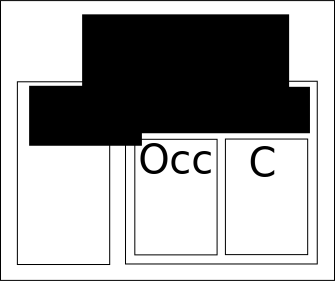
\includegraphics[width=6cm]{fm_index}
        \caption{Znázornenie štruktúry FM-indexu}
        \label{fig:fm_index}
    \end{figure}
    
    \subsubsection{Komprimované sufixové pole}
    Komprimované sufixové pole (\emph{CSA - compressed suffix array}) pole sa využíva na zistenie pozície daného podreťazca v texte $T$. Nie je si ale potrebné držať v ňom pozície všetkých sufixov $T$, keďže pomocou \emph{LF mappingu} vieme zrekonštruovať podreťazec $T$ začínajúci na ľubovoľnej pozícii. Preto si stačí pamätať len pozície niektorých sufixov a potom pomocou \emph{LF mappingu} len čiastočne rekonštruovať $T$, pokým nedosiahneme nejakú pamätanú pozíciu sufixu. Komprimované sufixové pole zaberá iba zlomok pamäte oproti pôvodnému, no na oplátku sa kvôli nutnosti čiastočnej rekonštrukcie výrazne zvýši čas trvania operácie \emph{locate}.
    
    \subsubsection{Tabuľka prefixových súm}
    Táto tabuľka obsahuje pre každý znak $c$ danej abecedy počet výskytov lexikograficky menších znakov ako $c$ v danom reťazci $S$. Narozdiel od sufixového poľa ale nie je tak ľahko komprimovateľná, keďže frekvencie výskytu jednotlivých znakov sú na sebe navzájom nezávislé. Na druhej strane, zvyčajne býva veľkosť abecedy rádovo menšia než dĺžka textu, takže veľkosť tejto tabuľky bude prispievať do celkovej pamäťovej náročnosti len malou časťou\footnote{Špeciálne to platí v našom, bioinformatickom kontexte, kde používame štvorpísmenovú abecedu a genómy majú dĺžky v miliónoch.}.
    
    \subsubsection{Tabuľka výskytov}
    Tabuľka výskytov $Occ$ pre dané $c$ a $k$ vráti počet výskytov znaku $c$ v prefixe $S[0..k]$ daného reťazca $S$. Keď túto tabuľku skonštruujeme nad $BWT(T)$, tak \emph{LF mapping} vieme zadefinovať ako $$LF(i) = C[BWT(T)[i]] + Occ(BWT(T)[i], i)$$
    Rýchlosť prístupu k tejto tabuľke a jej pamäťová náročnosť je najdôležitejším faktorom FM-indexu. 
    
    \bigskip
    
    Pre lepšiu predstavu uveďme príklad:
    
    \begin{example}
        \label{ex:fm_index}
        Nech $T = banana\$$, potom $BWT(T) = annb\$aa$. Tabuľky $C$ a $Occ$ skonštruované nad $BWT(T)$ potom vyzerajú nasledovne:
        
        \bigskip
        
        \begin{minipage}{2.5in}
            \begin{tabular}{ | c | c | c | c | c | }
                \multicolumn{5}{c}{\textbf{C pre \emph{annb\$aa}}} \\ \hline
                \textbf{c}    & \$ & a & b & n                     \\ \hline
                \textbf{C[c]} & 0  & 1 & 4 & 5                     \\ \hline
            \end{tabular}
        \end{minipage}
        \begin{minipage}{2.5in}
            \begin{tabular}{ | c | c | c | c | c | c | c | c | }
                \multicolumn{8}{c}{\textbf{Occ(c, k) pre \emph{annb\$aa}}} \\ \hline
                            & \textbf{a} & \textbf{n} & \textbf{n} & \textbf{b} & \textbf{\$} & \textbf{a} & \textbf{a} \\ \hline
                            & \textbf{0} & \textbf{1} & \textbf{2} & \textbf{3} & \textbf{4}  & \textbf{5} & \textbf{6} \\ \hline
                \textbf{\$} & 0          & 0          & 0          & 0          & 1           & 1 & 1 \\ \hline                 
                \textbf{a}  & 1          & 1          & 1          & 1          & 1           & 2 & 3 \\ \hline
                \textbf{b}  & 0          & 0          & 0          & 1          & 1           & 1 & 1 \\ \hline  
                \textbf{n}  & 0          & 1          & 2          & 2          & 2           & 2 & 2 \\ \hline
            \end{tabular}
        \end{minipage}
    \end{example}

    \subsection{Vyhľadávanie pomocou FM-indexu}
    Vyhľadávanie v FM-indexe rozdelíme na dve fázy - \emph{počítaciu} a \emph{lokalizačnú} (pri operácii \emph{count} stačí vykonať prvú časť, pre \emph{locate} obe). \emph{Počítacia} fáza má za úlohu identifikovať rozsah sufixov zo sufixového poľa, ktoré majú rovnaký prefix -- vyhľadávanú vzorku\footnote{Z definície sufixového poľa vyplýva, že sufixy s rovnakým prefixom nasledujú v sufixovom poli za sebou} a \emph{lokalizačná} fáza potom identifikuje vzorky v sufixovom poli.
    
    \subsubsection{Počítacia fáza}
    Hľadanie vzorky v sufixovom poli je časovo veľmi efektívne, pretože sa zároveň hľadajú všetky výskyty danej vzorky $P$ -- simultánnym posúvaním ukazovateľov hornej a dolnej hranice v sufixovom poli. Označme tieto ukazovatele $sp$ a $ep$ (z ang. \emph{starting} resp. \emph{ending pointer}). Znak $c$ bude obsahovať momentálne spracovávaný znak vzorky $P$, pričom začneme posledným znakom a budeme tiež využívať pomocné polia $Occ$ a $C$ zadefinované v predchádzajúcej časti. Ukazovateľ $sp$ bude inicializovaný na $C[c]$ a ukazovateľ $ep$ na $C[c + 1]$ -- v tomto prípade už tieto ukazovatele ukazujú na prvý resp. posledný výskyt posledného písmena $P$ v $F$\footnote{Pripomeňme, že $F$ je prvým stĺpcom $BWM$ a $F$ je vlastne pole znakov, ktoré zodpovedajú indexom sufixového poľa do pôvodného textu $T$.}.
    
    \bigskip
    
    \begin{pseudocode}[label=lst:fm_search_algorithm,caption={Algoritmus na hľadanie vzorky pomocou FM-indexu}]
i = P.length - 1
c = P[i]
sp = C[c]
ep = C[c + 1]

while i > 0 do
  i = i - 1
  c = P[i]
  sp = C[c] + Occ(c, sp - 1)
  ep = C[c] + Occ(c, ep) - 1
end
    \end{pseudocode}
    
    $Occ(c, sp - 1)$ (riadok 5) vracia počet znakov $c$ v $BWT(T)[0..(sp - 1)]$. Keď k nemu pripočítame počet znakov, ktoré sú menšie než $c$ ($C[c]$) dostávame pozíciu prvého $c$ v rozsahu $sp$ až $ep$ v $F$. Operácie v riadkoch 5 a 6 realizujú \emph{LF mapping} pre prvý a posledný výskyt $c$ v $BWT(T)[sp..ep]$ (ak by sme nemali k dispozícii tabuľku $Occ$, museli by sme najprv nájsť prvý a posledný výskyt $c$ v $BWT(T)[sp..ep]$ a až potom použiť \emph{LF mapping}).
    
    \bigskip
    \begin{example}
        Postup vyhľadávania vzorky $P = nan$ by vyzeral nasledovne: \\ \\
        \begin{minipage}{2in}
            \begin{tabular}{ c c c }
                \multicolumn{3}{c}{\emph{P = na\textbf{n}}} \\
                \textbf{F} &        & \textbf{L} \\
                \$         & \ldots & a          \\            
                a          & \ldots & n          \\
                a          & \ldots & n          \\
                a          & \ldots & b          \\
                b          & \ldots & \$         \\
                \textbf{n} & \ldots & a          \\ 
                \textbf{n} & \ldots & a          \\
            \end{tabular}
        \end{minipage}
        \begin{minipage}{2in}
            \begin{tabular}{ c c c }
                \multicolumn{3}{c}{\emph{P = n\textbf{an}}} \\
                \textbf{F} &        & \textbf{L} \\
                \$         & \ldots & a          \\            
                a          & \ldots & n          \\
                \textbf{a} & \ldots & n          \\
                \textbf{a} & \ldots & b          \\
                b          & \ldots & \$         \\
                n          & \ldots & a          \\ 
                n          & \ldots & a          \\
            \end{tabular}
        \end{minipage}
        \begin{minipage}{2in}
            \begin{tabular}{ c c c }
                \multicolumn{3}{c}{\emph{P = \textbf{nan}}} \\
                \textbf{F} &        & \textbf{L} \\
                \$         & \ldots & a          \\            
                a          & \ldots & n          \\
                a          & \ldots & n          \\
                a          & \ldots & b          \\
                b          & \ldots & \$         \\
                \textbf{n} & \ldots & a          \\ 
                n          & \ldots & a          \\
            \end{tabular}
        \end{minipage}
    \end{example}
    \bigskip

    \subsubsection{Lokalizačná fáza}
    Výsledkom počítacej fázy sú dva indexy, $sp$ a $ep$, ktoré vymedzujú rozsah v sufixovom poli textu $T$. A práve prvky prvky v tomto rozsahu nám prezradia, na ktorých pozíciach textu $T$ nastala zhoda s vyhľadávanou vzorkou.
    
    \subsubsection{Časová zložitosť}
    Časová zložitosť počítacej fázy je lineárna vzhľadom na dĺžku hľadanej vzorky $P$, keďže v každej iterácii spracujeme jeden znak $P$. Na druhej strane, dĺžka textu $T$ na túto operáciu vplyv nemá, preto je táto metóda mimoriadne vhodná na spracovávanie dlhých textov, ako sú napríklad genómy. Zložitosť počítacej fázy je tiež nezávislá na počte výskytov vzorky v texte, keďže hľadáme len hornú a dolnú hranicu výskytu. V každej iterácii tiež spravíme dva dotazy do tabuľky $Occ$, takže výsledný čas závisí tiež lineárne od časovej zložitosti dotazov na $Occ$.
    
    Pri časovej zložitosti lokalizačnej fázy je situácia opačná -- nezávisí na dĺžke hľadanej vzorky, ale na počte výskytov, keďže pre každý jeden musíme pristúpiť ku sufixovému poľu. Preto o zložitosti rozhoduje implementácia sufixového poľa.
    
    \subsubsection{Zlepšenia}
    Ak by mala tabuľka $Occ$ odpovedať v konštantnom čase, zaberala by značné množstvo pamäte, preto sa v praxi pri jej implementácii používajú sofistikovanejšie dátové štruktúry ako napríklad \emph{wavelet tree} \cite{GGV03}.
    
    Čo sa týka lokalizačnej fázy, tak je potrebné spomenúť, že pamätanie si celého sufixového poľa by zaberalo priveľa pamäte, preto sa v praxi používajú napríklad komprimované sufixové pole -- ukladá sa len časť pôvodného sufixového poľa a chýbajúce hodnoty sa potom v prípade potreby dorátavajú pomocou pamätaných hodnôt.
    
    \todo{MTF, RL, wavelet, huffman, ... citacie, odkazy, fm index v2}
    
\section{Algoritmy na zostavovanie genómu}
    Výsledkom sekvenovania genómu (pri použití súčasných technológií) je veľké
    množstvo malých fragmentov - \emph{sequencing reads}, ktoré je potrebné
    zostaviť do jednej súvislej sekvencie. Náročnosť tejto úlohy závisí najmä
    od:
    
    \begin{itemize}
        \item dĺžky zostavovaného genómu - čím je kratší, tým je to jednoduchšie
        \item dĺžok jednotlivých fragmentov - čím sú dlhšie, tým lepsie
        \item priemernej hĺbky pokrytia - tzn koľko fragmentov v priemere
        pokrýva konkrétnu pozíciu zostavovanej sekvencie - čím viac, tým lepšie
    \end{itemize}

    \subsection{Najkratšie spoločné nadslovo}
    Asi najjednodušiu formuláciu problému zostavovania genómu predstavuje
    problém hľadania najkratšieho spoločného nadslova (\emph{shortest common
    superstring}).
    
    \begin{defn}
        Najkratším spoločným nadslovom reťazcov $S_1, S_2, \ldots, S_k$ nazývame
        najkratší reťazec $S$ taký, že každé $S_i$ je podslovo $S$.
    \end{defn}
    
    Tento problém je ale NP-ťažký, takže nepoznáme žiadny rýchly algoritmus,
    ktorý vždy nájde riešenie. Jednoduchá heuristika by vyzerala nasledovne:
    
    \begin{itemize}
        \item nájdi také dva fragmenty, ktoré majú najväčší prekryv, t.j.
        najdlhšiu $\alpha$ takú, že $S_i = \alpha\beta$ a $S_j = \gamma\alpha$
        \item spoj $S_i$ a $S_j$ do $\gamma\alpha\beta$
        \item opakuj prvý krok, kým neozostane iba jedno slovo
    \end{itemize}
    
    O tomto algorime sa dá dokázať, že je to 3.5-aproximačný algoritmus, t.j.
    nájdené riešenie bude mať vždy dĺžku nanajvýš 3.5-násobku optimálnej dĺžky.
    Síce je problém najkratšieho spoločného nadslova pomerne elegantnou
    formuláciou problému zostavovania genómov, je tento problém príliš ťažký na
    to, aby bolo jeho riešenie praktické pre veľké genómy. Preto sa v praxi
    používajú iné metódy.

    \subsection{Overlap-Layout-Consensus}
    Táto metóda, ako už jej názov naznačuje, pracuje v troch fázach:
    
    \subsubsection{Overlap}
    V tejto fáze assembler hľadá navzájom sa prekrývajúce fragmenty a spája ich do dlhších fragmentov, \emph{kontigov}. 
    
    Porovnávanie každej dvojice fragmentov by však bolo v praxi veľmi časovo náročné, nakoľko fragmentov môžu byť často milióny a pri porovnaní každej dvojice by sme potrebovali rádovo $O(n^2k)$ času (kde $n$ je počet fragmentov a $O(k)$ je čas, ktorý trvá porovnanie dvoch fragmentov). 
    
    Efektívnejšie algoritmy sú založené na predpoklade, že ak sa dva fragmenty úplne zhodujú na úseku dľžky aspoň $k$ (v praxi sa používa $k \approx 24$ ), tak pochádzajú z toho istého miesta v sekvenovanom genóme a teda sú spojené do jedného kontigu. 
    
    Vo všeobecnosti vyzerá tento postup nasledovne:
    \begin{itemize}
        \item vytvor zoznam podreťazcov dĺžky $k$ zo všetkých fragmentov, pričom ku každému podreťazcu si zapamätaj, z ktorého fragmentu pochádza
        \item lexikograficky utrieď zoznam podreťazcov
        \item skupiny výrazne sa prekrývajúcich fragmentov sa v utriedenom zozname budú vyskytovať pohromade a práve to sú dobrí kandidáti na spojenie do kontigov
    \end{itemize}
    
    \subsubsection{Layouy}
V druhej fáze assembler určuje relatívnu polohu jednotlivých kontigov a ich približné vzdialenosti, výsledné bloky kontigov sa nazývajú \emph{superkontigy}.

    \subsubsection{Consensus}
V poslednej fáze je vytvorená finálna sekvencia superkontigov, ktorá pokrýva genóm (alebo aspoň jeho časti). 
\\ \\
Často sa ale zvykne používať aj grafová reprezentácia tohto algoritmu. Vrcholmi grafu sú fragmenty, hrana medzi vrcholmi je vtedy, ak sa tieto dva fragmenty prekrývajú (overlap). V layout fáze sa tento graf zjednodušuje (napr. vymazanie nadbytočných hrán). Fáza consensus potom spočíva v nájdení hamiltonovskej cesty v tomto grafe.
    
    \subsection{De Bruijnove grafy}
    Tento prístup využíva to, že (obvykle) máme pri sekvenovaní veľké množstvo
    dát, a preto si môžme dovoliť časť obsiahnutej informácie v nich
    odignorovať.
    
    Pre jednoduchosť budeme predpokladať, že všetky fragmenty pochádzajú z
    jedného vlákna a snažíme sa zostaviť len jeden, úplne pokrytý chromozóm.

    Algoritmus pre vytvorenie \emph{de Bruijnovho grafu} vyzerá nasledovne:
    
    \begin{itemize}
        \item vytvor zoznam všetkých podreťazcov dĺžky $k$ zo všetkých
        fragmentov ($k$-tice)
        \item vrcholy grafu budú tvoriť všetky úseky dĺžky $k - 1$ (teda
        podreťazce podreťazcov dĺžky $k$)
        \item jednotlivé $k$-tice budú reprezentované orientovanými hranami v
        grafe, pričom $k$-tica $s_1 s_2 \ldots s_k$ spája vrcholy $s_1 s_2
        \ldots s_{k-1}$ a $s_2 s_3 \ldots s_k$. 
    \end{itemize}
    
    Eulerovský ťah v takomto grafe potom predstavuje hľadaný genóm.
    
    \begin{example}
        Uvažujme fragmenty \texttt{CCTGCC} a \texttt{GCCACC} a $k = 3$. Zoznam
        $k$-tic teda bude vyzerať nasledovne:
        
        \bigskip
        
        \begin{tabular}{ c c }
            \textbf{CCTGCC} & \textbf{GCCACC} \\  
            \texttt{CCT}    & \texttt{GCC}    \\
            \texttt{CTG}    & \texttt{CCA}    \\
            \texttt{TGC}    & \texttt{CAC}    \\
            \texttt{GCC}    & \texttt{ACC}    \\
        \end{tabular}  
        
        \bigskip
        
        Úseky dĺžky $k-1$: \texttt{CC}, \texttt{CT}, \texttt{TG}, \texttt{GC},
        \texttt{CA}, \texttt{AA}, \texttt{AC}
        
        \bigskip
        
        Graf: 
        
        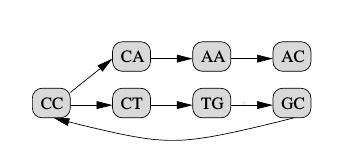
\includegraphics{graf.png}
    \end{example}